% =============================================================================
% Vozmezdie: narrative methods paper + technical appendix
% pdfLaTeX + BibTeX (Overleaf)
% =============================================================================
\documentclass[11pt,a4paper]{article}

\usepackage[T1]{fontenc}
\usepackage[utf8]{inputenc}
\usepackage{lmodern}
\usepackage{microtype}
\usepackage{geometry}
\geometry{margin=1in}

\usepackage{amsmath,amssymb,amsthm}
\usepackage{graphicx}
\usepackage{booktabs}
\usepackage{enumitem}
\usepackage[numbers,sort&compress]{natbib}
\usepackage{xcolor}

\usepackage{tikz}
\usetikzlibrary{arrows.meta,positioning,calc,fit}

\usepackage[hidelinks]{hyperref}

\newtheorem{theorem}{Theorem}[section]
\newtheorem{lemma}[theorem]{Lemma}
\newtheorem{proposition}[theorem]{Proposition}
\newtheorem{corollary}[theorem]{Corollary}
\theoremstyle{remark}
\newtheorem{remark}[theorem]{Remark}

\newcommand{\Sig}{\Sigma^\ast}
\newcommand{\Pred}{\mathrm{Pred}}
\newcommand{\GT}{\mathrm{GT}}

\title{Expert-Grounded LLM Evaluation on Declassified Ex-KGB Archival Documents:\\
The Vozmezdie Pipeline, Report Site, and Formal Specification}
\author{Sean Martin Lis\\
Canadian Institute of Ukrainian Studies (CIUS)}
\date{\textit{Draft / publication date to be inserted}}

\begin{document}
\maketitle

\section{Introduction}
\label{sec:intro}

\begin{center}
\fbox{\begin{minipage}{0.94\linewidth}
\textbf{Work in progress.}\quad
The introduction will be drafted separately (motivation, corpus framing, contributions, and how to read the report artefact). This placeholder marks the section as intentionally incomplete; citations and cross-references elsewhere in the paper remain active for drafting convenience.
\end{minipage}}
\end{center}

\vspace{1ex}
\noindent\textit{Roadmap.} Section~\ref{sec:abbrev} lists abbreviations and symbols; Section~\ref{sec:task} defines what a labelled segment is; Section~\ref{sec:methods} walks through ingest, prediction, alignment, and metrics (Figures~\ref{fig:alignment_sketch} and~\ref{fig:metrics_bits}); Section~\ref{sec:results} combines visualization guidance with a fixture-backed journey (Figures~\ref{fig:reading_loop}--\ref{fig:mismatch_top}) plus complementary agreement and length diagnostics (Figures~\ref{fig:fixture_agreement}--\ref{fig:ttr_axis}, Section~\ref{sec:fixture_balance}); later passages record limitations, contributions, and formal appendices. Figures~\ref{fig:segment_row} and~\ref{fig:dataflow_text} preview tabular structure before equations appear.

\section*{Related work}
Human specialists label text by choosing categories; naive ``percent agreement'' treats random guessing as skill. Cohen's coefficient $\kappa$ was introduced to subtract chance agreement for nominal scales \citep{cohen1960coefficient}. Carletta's tutorial connects $\kappa$ to language-engineering evaluation \citep{carletta1996assessing}. Pustejovsky and Stubbs, together with Gwet's handbook, explain annotation workflows where definitions drift and raters disagree legitimately \citep{pustejovsky2012natural,gwet2021handbook}; those references motivate pairing quantitative summaries with definitional transparency.

Modern sequence models generate text by repeatedly sampling the next token from a learned distribution \citep{vaswani2017attention}. Structured extraction benchmarks such as ExtractBench stress valid JSON outputs rather than eloquent prose because parsers discard malformed rows \citep{extractbench2026}. Digital-humanities pipelines likewise warn that OCR corrections propagate downstream \citep{norton2026ocrprovenance}. Together these strands justify documenting decode randomness, parser brittleness, and deterministic comparison separately. When dashboards invite many simultaneous comparisons, Benjamini--Hochberg style multiplicity control supplies a standard guardrail \citep{benjamini1995controlling}.

\tableofcontents
\newpage

\section*{Abbreviations and symbols}
\addcontentsline{toc}{section}{Abbreviations and symbols}
\label{sec:abbrev}

\noindent\textbf{Abbreviations.}\quad
The following short forms appear in the narrative or figures.

\begin{tabular}{@{}p{2.6cm}p{11.2cm}@{}}
\textbf{API} & Application programming interface (remote services invoked over the network). \\
\textbf{BH} & Benjamini--Hochberg procedure for multiplicity control when many comparisons are inspected. \\
\textbf{CI} & Continuous integration (automated test runs in the repository pipeline). \\
\textbf{CIUS} & Canadian Institute of Ukrainian Studies (author affiliation). \\
\textbf{CSV} & Comma-separated values (tabular interchange format for expert rows). \\
\textbf{EOS} & End-of-sequence token marking stop conditions during language-model decoding. \\
\textbf{GPU} & Graphics processing unit (local accelerator for neural inference). \\
\textbf{GT} & Ground truth: expert-supplied segment rows; typeset as $\GT$ when naming the loader map. \\
\textbf{HTML} & Hypertext Markup Language (static report output). \\
\textbf{HTTP} & Hypertext Transfer Protocol; \textbf{POST} denotes the request method used to call Ollama. \\
\textbf{JSON} & JavaScript Object Notation (serialized comparison payloads and model outputs). \\
\textbf{KGB} & Soviet state security agency (historical context for declassified memoranda). \\
\textbf{LLM} & Large language model (generative model producing candidate segment labels). \\
\textbf{NLP} & Natural language processing. \\
\textbf{OCR} & Optical character recognition (some catalogue texts originate from OCR pipelines). \\
\textbf{Pred} & Predictions: machine or merged assessment rows; typeset as $\Pred$ when naming the predictor map. \\
\textbf{RUS / ENG} & Russian and English document text fields resolved at ingest (also \textit{Rus.}\ in figures). \\
\textbf{SSR} & Soviet Socialist Republic (e.g.\ Ukrainian SSR). \\
\textbf{TTR} & Type-token ratio: distinct word types divided by total tokens (lexical diversity). \\
\textbf{UI} & User interface (taxonomy colours, glossary, readers in the report site). \\
\textbf{URL} & Uniform Resource Locator (document identifiers in hosted Voyant corpora). \\
\end{tabular}

\vspace{1.5ex}
\noindent\textbf{Symbols and notation.}\quad
Mathematical shorthand used in Section~\ref{sec:methods} and the appendices.

\begin{tabular}{@{}p{2.6cm}p{11.2cm}@{}}
$\Pi$ & End-to-end composed pipeline (Eq.~\eqref{eq:Pi}): ingest through HTML report. \\
$\circ$ & Composition of maps; $(f\circ g)(x)=f(g(x))$, applied right-to-left in Eq.~\eqref{eq:Pi}. \\
$\mathcal{M}$ & Index set for catalogue entries passed to ingest. \\
$\mathcal{C},\mathcal{F}$ & Finite sets of admissible content categories and framing strategies from taxonomy $T$. \\
$\Sig$ or $\Sigma^\ast$ & Space of finite-length strings (Unicode text fragments and prompts). \\
$\eta(\cdot)$ & Phrase normalization before alignment: strip, lowercase, collapse internal whitespace. \\
$\pi_{8000}(\cdot)$ & Truncation of Russian document text to the first 8000 Unicode characters in LLM prompts. \\
$\theta$ & Neural network weights for the served causal language model $\mathcal{A}_\theta$. \\
$\tau$ & Sampling temperature rescaling logits before softmax during decoding. \\
$u_t$ & Logit vector over vocabulary at decode step $t$. \\
$z_{1:t}$ & Token prefix generated up to step $t$. \\
$\kappa$ & Cohen's kappa (chance-corrected agreement for categorical labels). \\
$\bot$ & Sentinel for failed HTTP transport in the formal LLM interface sketch. \\
\end{tabular}

\newpage

% =============================================================================
\section{The task}
\label{sec:task}

We ask whether an automated assistant can mimic expert archivists who tag short spans with two labels drawn from closed lists. Each span becomes one table row: identifiers, Russian wording (English when provided), a \emph{content category} such as Actors or Places, and a \emph{framing strategy} such as Institutional / Bureaucratic Lingo or Ideological Framing (Discrediting). Naming those lists up front turns subjective judgment into reproducible targets so auditors can reopen individual rows instead of debating abstract totals.

Content and framing answer different questions on purpose. Content records what entities or facts the span inventories; framing records how those facts are rhetorically packaged (neutral roster language versus ideological shading, for instance). Secret-police memoranda frequently stack factual lists with evaluative casing, so merging both questions into one tag would erase distinctions historians rely on.

Canonical ids and colours ship with the taxonomy file; optional glossary prose merges into the report when configured.\footnote{Older drafts sometimes renamed categories; stored rows keep canonical ids so the comparator compares consistent strings.}

Qualifiers and examples therefore surface beside segments inside the generated website so readers can see \emph{why} experts and models diverged rather than inferring motives from a scalar alone.

\begin{figure}[htbp]
\centering
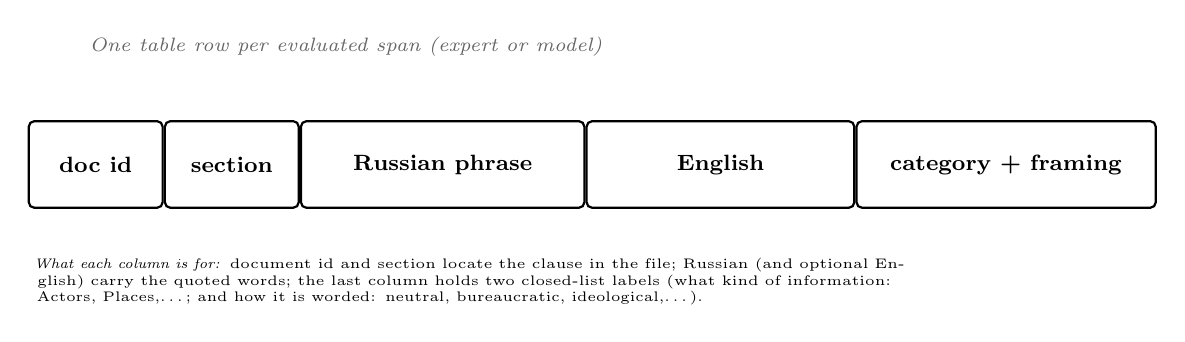
\begin{tikzpicture}[
  font=\footnotesize,
  >=Stealth,
  hdr/.style={font=\scriptsize\itshape,text=black!60},
  cell/.style={draw,thick,rounded corners=2pt,minimum height=11mm,align=center,inner sep=4pt},
]
\node[hdr,anchor=south west] at (-0.2,1.25) {One table row per evaluated span (expert or model)};
\node[cell,minimum width=17mm] (n1) at (0,0) {\textbf{doc id}};
\node[cell,minimum width=17mm,anchor=west] (n2) at (n1.east) {\textbf{section}};
\node[cell,minimum width=36mm,anchor=west] (n3) at (n2.east) {\textbf{Russian phrase}};
\node[cell,minimum width=34mm,anchor=west] (n4) at (n3.east) {\textbf{English}};
\node[cell,minimum width=38mm,anchor=west] (n5) at (n4.east) {\textbf{category + framing}};
\node[below=5mm of n1.south west,anchor=north west,font=\tiny,text width=0.92\textwidth,align=left]
  {\textit{What each column is for:} document id and section locate the clause in the file; Russian (and optional English) carry the quoted words; the last column holds two closed-list labels (what kind of information: Actors, Places,\ldots; and how it is worded: neutral, bureaucratic, ideological,\ldots).};
\end{tikzpicture}
\caption{Conceptual shape of a segment row: identifiers and prose slots feed comparison; both taxonomy strings must match (after trimming) for a full agreement.}
\label{fig:segment_row}
\end{figure}

\begin{figure}[htbp]
\centering
\begin{minipage}{0.96\linewidth}
\centering
\begin{tikzpicture}[
  font=\footnotesize,
  >=Stealth,
  step/.style={
    draw,
    rounded corners=3pt,
    align=left,
    inner sep=9pt,
    text width=\linewidth,
  },
]
\node[step] (rus) {\textbf{Source.}\par Memorandum text (Russian primary; English when listed).};
\node[step,below=9mm of rus.south] (ing) {\textbf{Ingest.}\par Match catalogue entries to files and ids.};
\node[step,below=9mm of ing.south] (gtb)
  {\textbf{Expert table ($\GT$).}\par Ordered rows from historians: each row is one Russian snippet plus topic and framing labels.};
\node[step,below=9mm of gtb.south] (prb)
  {\textbf{Prediction table ($\Pred$).}\par Same columns filled by an LLM, the CI stub, or merged blind JSON.};
\node[step,below=9mm of prb.south] (cmp)
  {\textbf{Compare.}\par Normalize snippets, pair expert vs.\ model rows, mark category/framing match.};
\node[step,below=9mm of cmp.south] (out)
  {\textbf{Website output.}\par Tables, charts, glossary links back to segments.};
\draw[thick,-Stealth] (rus.south)--(ing.north);
\draw[thick,-Stealth] (ing.south)--(gtb.north);
\draw[thick,-Stealth] (gtb.south)--(prb.north);
\draw[thick,-Stealth] (prb.south)--(cmp.north);
\draw[thick,-Stealth] (cmp.south)--(out.north);
\end{tikzpicture}
\end{minipage}
\caption{End-to-end flow drawn as a vertical ribbon so each stage gets the full column width. Expert and model tables are parallel in code but stacked here to avoid cramped side-by-side boxes.}
\label{fig:dataflow_text}
\end{figure}

% =============================================================================
\section{Methods and approach}
\label{sec:methods}

\subsection{Pipeline overview}
The shipped software loads archival texts, asks either a human workflow or a language model to fill segment tables, loads expert tables, pairs rows, writes a JSON bundle, and builds static HTML. Equation~\eqref{eq:Pi} is only shorthand for that ordering: each named stage is a deterministic program step except the neural decode itself.

Reading the equation once avoids rereading five paragraphs. $\mathrm{Ingest}$ loads catalogue entries into payloads $(\mathrm{id},\mathrm{RUS},\mathrm{ENG},\ldots)$. $\Pred$ is whichever routine produced machine rows (LLM, test stub, or merged human JSON); $\GT$ loads expert rows from HTML/CSV/JSON; both read the same ingested files before comparison. $\mathrm{Compare}$ aligns Russian phrases and writes match flags; $\mathrm{Serialize}$ freezes results to disk; $\mathrm{Report}$ renders the website. The symbol $\circ$ means ``apply in sequence,'' right-to-left as $(f\circ g)(x)=f(g(x))$, so ingest happens before HTML appears.

Fixing configuration and taxonomy, the shipped orchestrator realizes the composed pipeline $\Pi$:
\begin{equation}
\label{eq:Pi}
\Pi \;=\; \mathrm{Report}\;\circ\;\mathrm{Serialize}\;\circ\;\mathrm{Compare}\;\circ\;\bigl(\GT,\,\Pred\bigr)\;\circ\;\mathrm{Ingest}.
\end{equation}
Figure~\ref{fig:pipeline0} sketches module-level composition; Figures~\ref{fig:segment_row}--\ref{fig:dataflow_text} show how prose becomes aligned rows before math notation appears.

\begin{figure}[htbp]
\centering
\begin{minipage}{0.96\linewidth}
\centering
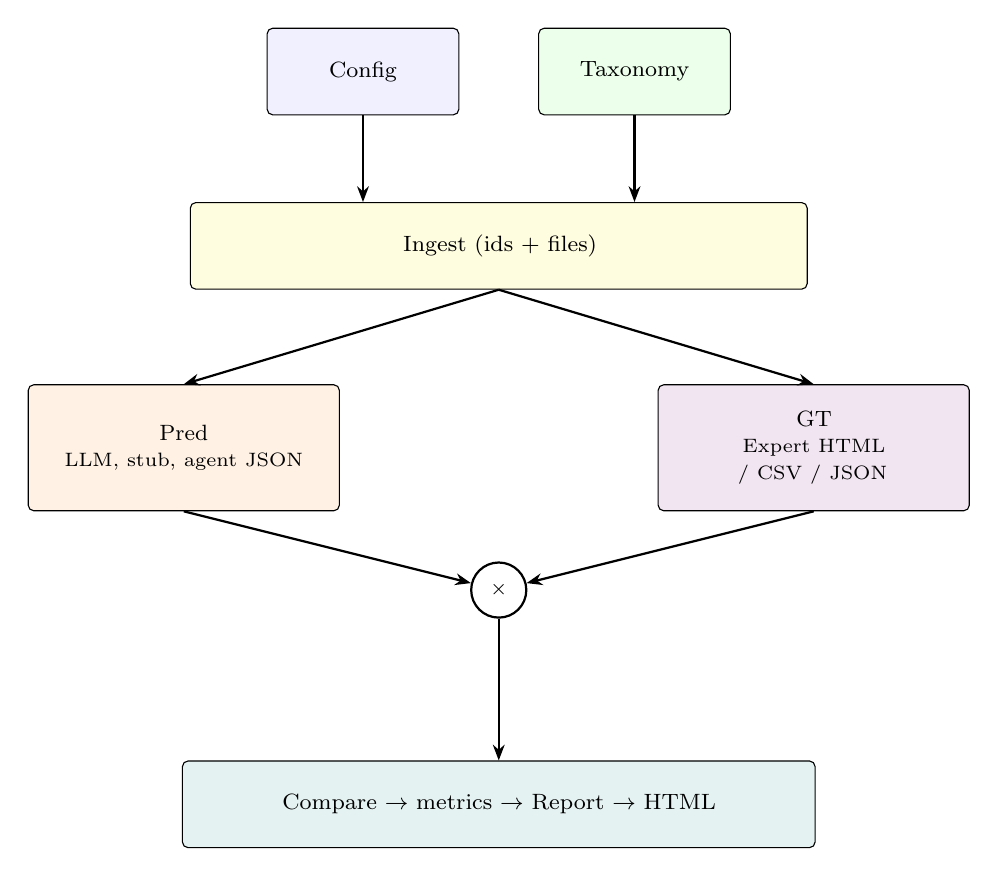
\begin{tikzpicture}[
  font=\footnotesize,
  box/.style={draw,rounded corners=2pt,minimum height=11mm,align=center,
    fill=gray!6},
  branch/.style={draw,rounded corners=2pt,text width=36mm,minimum height=16mm,align=center,inner sep=5pt},
  arr/.style={-{Stealth[length=2mm]},thick},
  >=Stealth,
]
\node[box,text width=22mm,fill=blue!6] (cfg) {Config};
\node[box,text width=22mm,right=10mm of cfg,fill=green!8] (tax) {Taxonomy};
\path ($(cfg.south)!0.5!(tax.south)$) coordinate (topmid);
\node[box,below=11mm of topmid,text width=76mm,fill=yellow!12] (ing) {Ingest (ids + files)};
\node[branch,anchor=north,fill=orange!10] (pred) at ($(ing.south)+(-40mm,-12mm)$)
  {$\Pred$\par\scriptsize LLM, stub, agent JSON};
\node[branch,anchor=north,fill=violet!10] (gt) at ($(ing.south)+(40mm,-12mm)$)
  {$\GT$\par\scriptsize Expert HTML / CSV / JSON};
\node[circle,draw,thick,fill=white,minimum size=7mm,inner sep=0pt] (merge)
  at ($(pred.south)!0.5!(gt.south)+(0,-10mm)$) {\scriptsize$\times$};
\node[box,below=18mm of merge,text width=78mm,fill=teal!10] (cmp)
  {Compare $\rightarrow$ metrics $\rightarrow$ Report $\rightarrow$ HTML};
\draw[arr] (cfg.south)--(cfg.south |- ing.north);
\draw[arr] (tax.south)--(tax.south |- ing.north);
\draw[arr] (ing.south)--(pred.north);
\draw[arr] (ing.south)--(gt.north);
\draw[arr] (pred.south)--(merge);
\draw[arr] (gt.south)--(merge);
\draw[arr] (merge)--(cmp.north);
\end{tikzpicture}
\end{minipage}
\caption{High-level composition $\Pi$ from Eq.~\eqref{eq:Pi}. Both branches receive ingest output; the circle marks where paired rows feed Compare.}
\label{fig:pipeline0}
\end{figure}

\subsection{Ingestion and bilingual texts}
Russian originals anchor token surfaces that downstream extractors segment; aligned English enables bilingual readers and English-only corpus charts without pretending translations were produced outside the catalogue. Each catalogue entry $i\in\mathcal{M}$ resolves deterministically to $(\mathrm{id}_i,\mathrm{RUS}_i,\mathrm{ENG}_i,\ldots)$ even when filenames contain spaces or alternate spellings, which matters because pairing keys on normalized Russian strings. Appendix~\ref{app:formal} abbreviates that resolver as $\mathrm{Ingest}(\mathcal{M})$.

\subsection{Prediction: extraction modes}
Three interchangeable producers feed $\mathrm{Compare}$:
\begin{enumerate}[leftmargin=*]
  \item \textbf{Local LLM via Ollama.} The adapter POSTs to Ollama without streaming. The prompt embeds $\pi_{8000}(\mathrm{RUS}_i)$, operator notation for ``truncate Russian document $i$ after the first 8000 Unicode characters.'' That ceiling is evidence of a pragmatic context budget, not a linguistic theory; anything past character 8000 never influences model logits while experts may still label tail spans. Returned free text is scanned for JSON lines; malformed lines disappear at parse time; empty parses fall back to the stub below.
  \item \textbf{Deterministic stub.} When CI fixtures run without weights, a heuristic splitter emits up to twenty-five phrases of length $\ge 4$ characters and cycles taxonomy codes. Evidence that rows came from the stub is visible as patterned categories; the implication is that stub metrics measure plumbing, not archival understanding.
  \item \textbf{Agent assessments.} Human annotators merge JSON keyed by document id after blind exports or scripted merges, letting $\Pred$ denote blended expert judgments instead of machine outputs when studies require it.
\end{enumerate}

Studies that must preserve expert boundaries exactly export segment lists without labels, then classify each fixed segment with prompts listing admissible categories and framings; latency is typically a few seconds per segment on local GPUs. Document-wide JSON extraction lets the model invent boundaries; per-segment classification freezes boundaries supplied by historians. Pooling confusion matrices across those regimes without disclosure would mix incomparable denominators, so papers should name which path instantiated $\Pred$.

\subsection{Ground truth and alignment}
Experts emit ordered rows $\GT(i)$ mirroring the prediction schema. Before comparing texts, the comparator applies $\eta(\cdot)$ to Russian phrases: strip surrounding whitespace, lowercase letters, collapse interior whitespace to single spaces. Evidence for $\eta$ appears in logs when ``Foo bar'' pairs with ``foo  bar''; evidence against fuzzy matching is that near-paraphrases remain apart unless one normalized span contains the other with length $\ge 4$ on the shorter side. Greedy passes pair exact $\eta$-matches first, then containment pairs; neither pass solves the globally optimal assignment problem \citep{kuhn1955hungarian}, yet fixed traversal yields reproducible audits valued here over maximal pairing counts. Appendix~\ref{app:compare} proves bookkeeping lemmas (no duplicated partners; accuracy denominators match paired rows).

\begin{figure}[htbp]
\centering
\begin{tikzpicture}[
  font=\scriptsize,
  >=Stealth,
  col/.style={text width=44mm,align=left,inner sep=4pt},
]
\node[col,draw] (gt1) {\textbf{Expert} $\GT$\quad row 1\\\textit{Rus.:} \ldots\textsf{гражданин Франции}\ldots\\\textit{Cat.:} Actors | \textit{Fram.:} Inst.\ bureaucratic};
\node[col,draw,below=5mm of gt1] (gt2) {\textbf{Expert} $\GT$\quad row 2\\\textit{Rus.:} \ldots\textsf{бухгалтерия}\ldots\\\textit{Cat.:} Actions | \textit{Fram.:} Action-focused};
\node[col,draw,right=22mm of gt1] (pd1) {\textbf{Model} $\Pred$\quad row A\\\textit{Rus.:} \ldots\textsf{гражданин франции}\ldots\\\textit{Cat.:} Actors | \textit{Fram.:} Generic neutral};
\node[col,draw,below=5mm of pd1] (pd2) {\textbf{Model} $\Pred$\quad row B\\\textit{Rus.:} \ldots\textsf{учётный отдел}\ldots\\\textit{Cat.:} Actions | \textit{Fram.:} Action-focused};
\draw[thick,blue!70!black,-Stealth] (gt1.east) -- node[above=1pt,font=\tiny]{paired via $\eta$} (pd1.west);
\node[below=2mm of gt2.south west,anchor=north west,font=\tiny,text width=108mm]
  {\textit{Illustration only:} expert row 2 and model row B use different Russian lemmas (\textsf{бухгалтерия} vs.\ \textsf{учётный отдел}), so no pairing edge is drawn until containment rules apply or rows stay orphaned. Row 1 pairs despite casing because $\eta$ lowercases both phrases. After pairing, row 1 yields category match $=1$, framing match $=0$ (strings differ on framing).};
\end{tikzpicture}
\caption{Simplified alignment sketch (not to scale): casing-only differences can still $\eta$-match; paraphrases break pairing even when labels partially agree. Compare applies ordered greedy rules to the full tables.}
\label{fig:alignment_sketch}
\end{figure}

\subsection{Metrics and the interactive report}
Agreement metrics are elementary counts once pairing exists: for each paired row we ask whether trimmed category strings match and whether trimmed framing strings match, recording ones or zeros; headline percentages average those bits and also report the conjunction (both match). Evidence lives in exported JSON beside each row; explainability demands pairing rows before interpreting percentages because unmatched spans contribute zero to agreement numerators while still signaling systemic failure. Serialized bundles drive static HTML tables, bilingual highlights sorted like expert tables, glossary tabs, and Research Lab charts whose expandable notes repeat the generator formulas. Aggregate charts remain illustrative secondary summaries \citep{carletta1996assessing,gwet2021handbook}: readers should descend to aligned rows whenever a figure surprises them.

\begin{figure}[htbp]
\centering
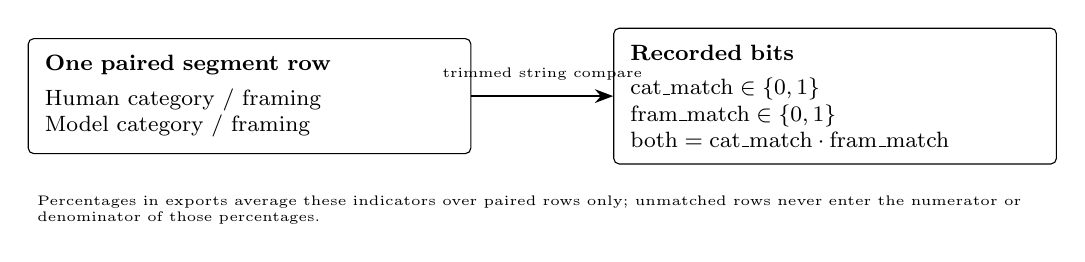
\begin{tikzpicture}[
  font=\footnotesize,
  >=Stealth,
  paired/.style={draw,rounded corners=2pt,inner sep=6pt,align=left,text width=52mm},
]
\node[paired] (pr)
  {\textbf{One paired segment row}\\[3pt]
   Human category / framing\\
   Model category / framing};
\node[paired,right=18mm of pr] (bits)
  {\textbf{Recorded bits}\\[3pt]
   $\mathrm{cat\_match}\in\{0,1\}$\\
   $\mathrm{fram\_match}\in\{0,1\}$\\
   $\mathrm{both}= \mathrm{cat\_match}\cdot\mathrm{fram\_match}$};
\draw[thick,-Stealth] (pr.east) -- node[above=2pt,font=\tiny]{trimmed string compare} (bits.west);
\node[below=4mm of pr.south west,anchor=north west,font=\tiny,text width=125mm]
  {Percentages in exports average these indicators over paired rows only; unmatched rows never enter the numerator or denominator of those percentages.};
\end{tikzpicture}
\caption{After alignment (Figure~\ref{fig:alignment_sketch}), agreement reduces to row-wise equality checks on taxonomy strings.}
\label{fig:metrics_bits}
\end{figure}

% =============================================================================
\section{Choices, challenges, successes, and limitations}
\label{sec:challenges}

This section names failure modes in the order they typically disturb interpretation: errors appear while text is being generated, while spans are being cut, while phrases are being paired, and while categories are being judged. Figure~\ref{fig:error_sources} summarizes that stack; each subsection below follows the same pattern: what breaks, what you would see in the exported tables or orphan counts, and why headline percentages alone mislead.

\begin{figure}[htbp]
\centering
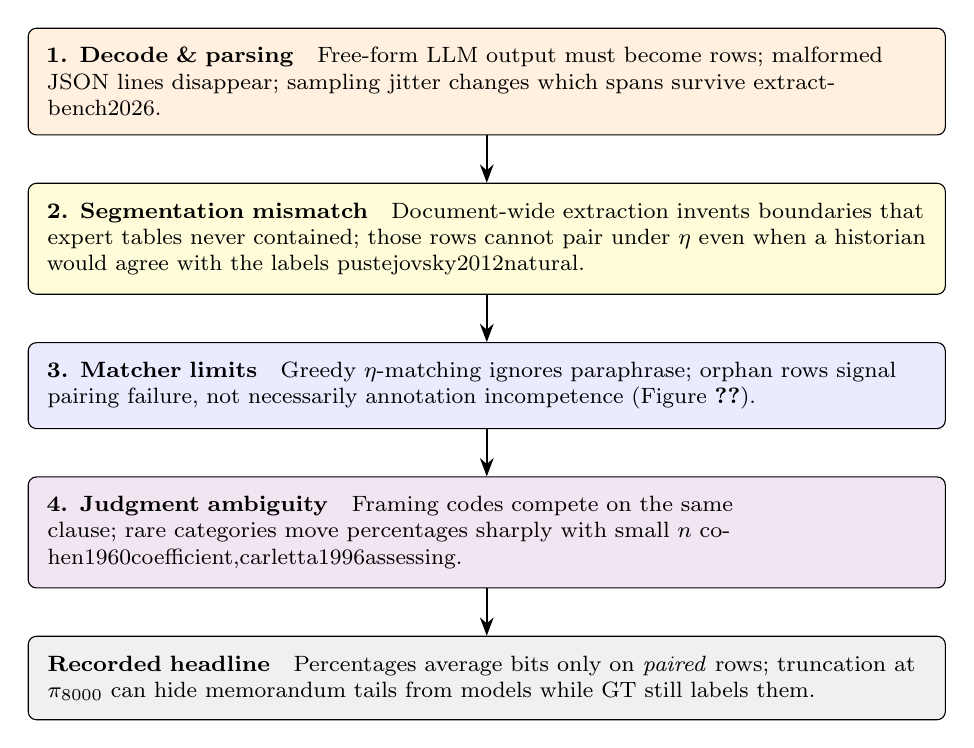
\begin{tikzpicture}[
  font=\footnotesize,
  >=Stealth,
  layer/.style={draw,rounded corners=3pt,align=left,inner sep=7pt,text width=0.92\textwidth},
]
\node[layer,fill=orange!12] (L1)
  {\textbf{1. Decode \& parsing}\quad Free-form LLM output must become rows; malformed JSON lines disappear; sampling jitter changes which spans survive \citep{extractbench2026}.};
\node[layer,below=6mm of L1,fill=yellow!15] (L2)
  {\textbf{2. Segmentation mismatch}\quad Document-wide extraction invents boundaries that expert tables never contained; those rows cannot pair under $\eta$ even when a historian would agree with the labels \citep{pustejovsky2012natural}.};
\node[layer,below=6mm of L2,fill=blue!8] (L3)
  {\textbf{3. Matcher limits}\quad Greedy $\eta$-matching ignores paraphrase; orphan rows signal pairing failure, not necessarily annotation incompetence (Figure~\ref{fig:alignment_sketch}).};
\node[layer,below=6mm of L3,fill=violet!10] (L4)
  {\textbf{4. Judgment ambiguity}\quad Framing codes compete on the same clause; rare categories move percentages sharply with small $n$ \citep{cohen1960coefficient,carletta1996assessing}.};
\node[layer,below=6mm of L4,fill=gray!12] (L5)
  {\textbf{Recorded headline}\quad Percentages average bits only on \emph{paired} rows; truncation at $\pi_{8000}$ can hide memorandum tails from models while $\GT$ still labels them.};
\draw[thick,-Stealth] (L1.south)--(L2.north);
\draw[thick,-Stealth] (L2.south)--(L3.north);
\draw[thick,-Stealth] (L3.south)--(L4.north);
\draw[thick,-Stealth] (L4.south)--(L5.north);
\end{tikzpicture}
\caption{Where disagreement enters before a reader ever opens a chart: decode noise and segmentation happen upstream of $\eta$ pairing; pairing limits sit upstream of trimmed label equality.}
\label{fig:error_sources}
\end{figure}

\subsubsection{Alignment sensitivity}
\textbf{Point.} Pairing is deliberately literal about Russian surface strings.

\textbf{Evidence.} Normalization $\eta$ fixes casing and whitespace but not synonyms; models that paraphrase headquarters accounting as \textsf{учётный отдел} while experts wrote \textsf{бухгалтерия} leave rows unpaired in Figure~\ref{fig:alignment_sketch}-style situations.

\textbf{Teach-back.} When mismatch flows spike (Section~\ref{sec:fixture_journey}), open the alignment column first: otherwise you interpret framing swaps that never belonged to the same segment.

\subsubsection{Framing subjectivity and skewed margins}
\textbf{Point.} Ideological versus bureaucratic readings can both sound plausible to a fluent reader.

\textbf{Evidence.} The bundled fixture's dominant heatmap cells stack hundreds of actor and action segments under ideology or bureaucracy (Figure~\ref{fig:heatmap_topcells}); a handful of Legal Framework rows moves document-level rates sharply.

\textbf{Teach-back.} Pair Cohen's $\kappa$ or confusion matrices with narrative gloss so skewed priors do not masquerade as model mastery \citep{cohen1960coefficient,carletta1996assessing}.

\subsubsection{Archival register}
\textbf{Point.} Memoranda blend factual inventory with evaluative casing aimed at party readers.

\textbf{Evidence.} Dual codes force models to recover both inventory (Actors, Actions) and posture (discrediting vs.\ institutional).

\textbf{Teach-back.} Expect systematic framing errors even when entity spans look easy; off-diagonal framing counts in Figure~\ref{fig:mismatch_top} quantify those swaps.

\subsubsection{What shipped successfully}
Deterministic comparison plus static HTML lets outsiders replay the same pairing logic years later; blind segment exports mitigate anchoring when fresh coders avoid seeing $\GT$ strings prematurely \citep{pustejovsky2012natural}.

\subsubsection{Structural limitation on extraction mode}
Document-wide JSON extraction and per-segment classification answer different scientific questions; pooling their confusion summaries without a methods footnote mixes incompatible segment populations \citep{extractbench2026}.

% =============================================================================
\section{Study effort and visualization-led reading}
\label{sec:results}

\subsection{Human labour}
Expert coding, review, and reconciliation consumed roughly 324 hours on the corpus shipped beside this framework. That number is not ornamentation: every downstream graphic collapses weeks of clause-by-clause judgment into a handful of curves, so treating charts as standalone evidence would erase the labour they summarize.

\subsection{A reader's journey through the bundled fixture}
\label{sec:fixture_journey}

Unless noted otherwise, this subsection describes the bundled sixteen-document sample referenced in the manuscript ($933$ segments, counted the same way the public Research Lab totals rows). Think of the journey as climbing a ladder: labour produced rows, rows produced paired comparisons, comparisons produced serialized metrics, metrics fed each Research Lab panel.

\textbf{Step A (coverage).} Sixteen memoranda surface as document identifiers in the comparison payload; $933$ segments enter corpus-wide tallies the same way the live report aggregates them.

\textbf{Step B (joint prevalence).} Before asking whether models agree, inspect what historians actually coded most often. Figure~\ref{fig:heatmap_topcells} ranks the five densest category$\times$framing cells; the modal pattern stacks Actors under ideological discrediting ($159$ segments), then Actors under institutional lingo ($118$), then action-heavy framings on Actions rows. Those magnitudes explain why framing errors sting even when entity spans look easy: the corpus spends enormous mass precisely where tone and inventory intertwine.

\textbf{Step C (where framing swaps concentrate).} Figure~\ref{fig:mismatch_top} lists the dominant off-diagonal directions in the framing mismatch matrix used by the site. The strongest asymmetry is institutional-on-model versus action-focused-on-human ($87$ paired segments), followed by the reverse swap ($35$), then institutional-on-model versus ideological-discrediting-on-human ($26$). Reading those integers beside the figure teaches a qualitative lesson: models soften drama into bureaucracy or vice versa more often than they confuse neutral with normalizing ideology.

\textbf{Step D (length is not the culprit).} Among segments whose $\max(|\mathrm{entry\_eng}|,|\mathrm{entry\_rus}|)\ge 50$ characters, mean lengths sit at $72.7$ characters when both category and framing agree ($n=112$) and $72.6$ when they disagree ($n=89$). The near equality hints that failures concentrate in ambiguous wording rather than oversized clauses. Figure~\ref{fig:length_mismatch_bins} stratifies paired-row \emph{counts} across coarse $\max$-length buckets so the $\ge 50$ slice is not the only visible regime.

\textbf{Step E (lexical diversity vs accuracy).} Section~\ref{sec:fixture_balance} resumes after Step~C's asymmetric swaps with headline agreement bars, then length-stratified disagreement counts, and finally document-level type-token spread (Figure~\ref{fig:ttr_axis}). English ratios span $0.403$--$0.643$ (mean $0.518$); repetitive bulletins can look ``simple'' stylistically while remaining hard semantically, so diversity plots work best as texture diagnostics, not proxies for model score.

\textbf{Step F (rhetorical twins).} Cosine similarity on framing-proportion vectors peaks at $0.998$ between catalogue documents \texttt{1213.txt} and \texttt{1245.txt}. Those files need not sit next to each other in archival ordering; similarity here measures rhetorical mixture, not fond proximity.

Figure~\ref{fig:reading_loop} closes the loop: aggregate charts remain trustworthy only when readers can drop to aligned rows and Voyant readers for context.

\begin{figure}[htbp]
\centering
\begin{tikzpicture}[font=\footnotesize,>=Stealth,
  step/.style={draw,rounded corners=2pt,minimum width=52mm,minimum height=10mm,align=center}]
\node[step,fill=blue!8] (s1) {Expert labour ($\approx 324$\,h)};
\node[step,below=7mm of s1,fill=blue!8] (s2) {$16$ memoranda, $933$ counted segments};
\node[step,below=7mm of s2,fill=blue!8] (s3) {Serialized comparison (paired rows + flags)};
\node[step,below=7mm of s3,fill=blue!8] (s4) {Research Lab charts};
\node[step,below=7mm of s4,fill=blue!8] (s5) {Comparison tables and Voyant readers};
\draw[-Stealth,thick] (s1)--(s2)--(s3)--(s4)--(s5);
\end{tikzpicture}
\par\vspace{2mm}
{\footnotesize Each stage stays tied to real quotations: charts aggregate table rows, and rows retain document and segment identifiers for drill-down.}
\caption{Fixture-centred reading order: anchor aggregates to serialized comparisons, then reopen bilingual rows or Voyant panels.}
\label{fig:reading_loop}
\end{figure}

\begin{figure}[htbp]
\centering
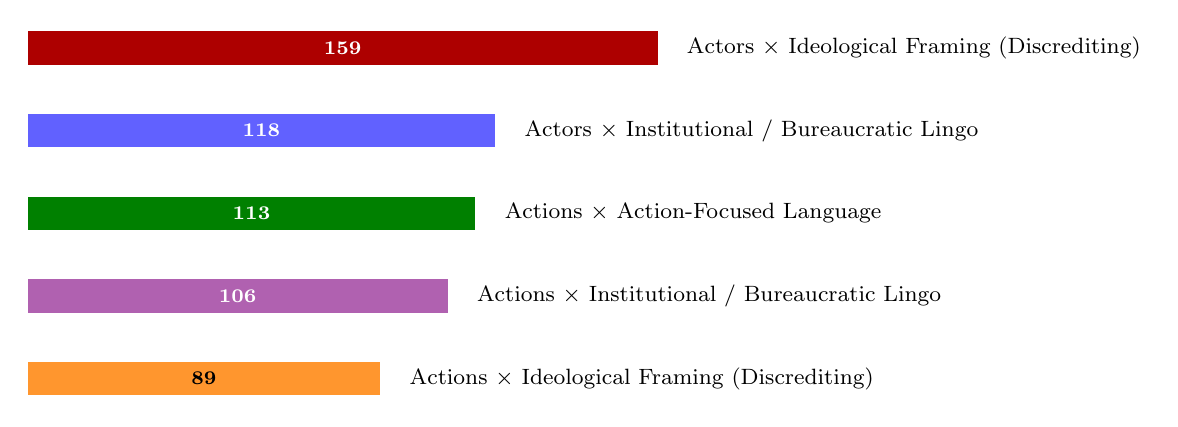
\begin{tikzpicture}[font=\footnotesize,y=0.42cm]
\pgfmathsetmacro{\BarUnit}{8/159}
% Distinct fills per row so ranks stay visually separable in print.
\coordinate (hb159) at ({159*\BarUnit},0.5);
\fill[red!68!black] (0,0) rectangle ({159*\BarUnit},1) node[midway,text=white,font=\scriptsize\bfseries] {159};
\node[anchor=west,font=\footnotesize] at ($(hb159)+(0.25,0)$) {Actors $\times$ Ideological Framing (Discrediting)};
\coordinate (hb118) at ({118*\BarUnit},-2);
\fill[blue!62] (0,-2.5) rectangle ({118*\BarUnit},-1.5) node[midway,text=white,font=\scriptsize\bfseries] {118};
\node[anchor=west,font=\footnotesize] at ($(hb118)+(0.25,0)$) {Actors $\times$ Institutional / Bureaucratic Lingo};
\coordinate (hb113) at ({113*\BarUnit},-4.5);
\fill[green!50!black] (0,-5) rectangle ({113*\BarUnit},-4) node[midway,text=white,font=\scriptsize\bfseries] {113};
\node[anchor=west,font=\footnotesize] at ($(hb113)+(0.25,0)$) {Actions $\times$ Action-Focused Language};
\coordinate (hb106) at ({106*\BarUnit},-7);
\fill[violet!62] (0,-7.5) rectangle ({106*\BarUnit},-6.5) node[midway,text=white,font=\scriptsize\bfseries] {106};
\node[anchor=west,font=\footnotesize] at ($(hb106)+(0.25,0)$) {Actions $\times$ Institutional / Bureaucratic Lingo};
\coordinate (hb89) at ({89*\BarUnit},-9.5);
\fill[orange!82] (0,-10) rectangle ({89*\BarUnit},-9) node[midway,text=black,font=\scriptsize\bfseries] {89};
\node[anchor=west,font=\footnotesize] at ($(hb89)+(0.25,0)$) {Actions $\times$ Ideological Framing (Discrediting)};
\end{tikzpicture}
\caption{Top five category$\times$framing cells in the bundled fixture (counts shared with the Research Lab heatmap). Each rank uses a distinct hue; bar length still scales linearly with count.}
\label{fig:heatmap_topcells}
\end{figure}

\begin{figure}[htbp]
\centering
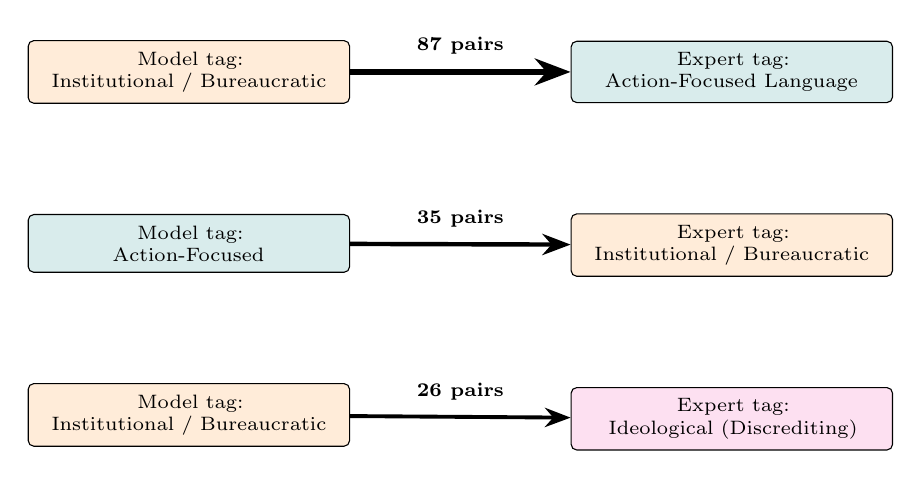
\begin{tikzpicture}[font=\footnotesize,>=Stealth,
  tag/.style={draw,rounded corners=2pt,inner sep=4pt,font=\scriptsize,text width=38mm,align=center}]
\node[tag,fill=orange!15] (mmA) {Model tag:\\Institutional / Bureaucratic};
\node[tag,right=28mm of mmA,fill=teal!15] (mmB) {Expert tag:\\Action-Focused Language};
\draw[line width=2.2pt,-Stealth] (mmA)--node[above=2pt,font=\scriptsize\bfseries]{87 pairs} (mmB);
\node[tag,below=14mm of mmA,fill=teal!15] (mmC) {Model tag:\\Action-Focused};
\node[tag,below=14mm of mmB,fill=orange!15] (mmD) {Expert tag:\\Institutional / Bureaucratic};
\draw[line width=1.6pt,-Stealth] (mmC)--node[above=2pt,font=\scriptsize\bfseries]{35 pairs} (mmD);
\node[tag,below=14mm of mmC,fill=orange!15] (mmE) {Model tag:\\Institutional / Bureaucratic};
\node[tag,below=14mm of mmD,fill=magenta!12] (mmF) {Expert tag:\\Ideological (Discrediting)};
\draw[line width=1.4pt,-Stealth] (mmE)--node[above=2pt,font=\scriptsize\bfseries]{26 pairs} (mmF);
\end{tikzpicture}
\caption{Three dominant off-diagonal framing swaps in the fixture mismatch-flow matrix (counts exclude diagonal agreements). Thicker arrows emphasize the bulk asymmetry.}
\label{fig:mismatch_top}
\end{figure}

\subsection{Fixture diagnostics after mismatch emphasis}
\label{sec:fixture_balance}

Figure~\ref{fig:mismatch_top} foregrounds directional framing swaps; paired-row summaries supply the complementary ledger. Aggregates below were recomputed from \texttt{docs/fixtures/comparison\_results.json} by scanning every document block's \texttt{aligned\_rows} list ($933$ paired rows across sixteen memoranda).

\subsubsection{Headline agreement on paired rows}
Category labels match on $677$ rows ($72.6\%$), framing labels on $711$ rows ($76.2\%$), and both jointly on $547$ rows ($58.6\%$). Framing agreement edges category agreement because tone labels sometimes stabilize even when inventory categories disagree; joint hits therefore sit materially lower than either margin alone. Figure~\ref{fig:fixture_agreement} keeps those three proportions visible beside the swap arrows so readers retain a sense of where greedy pairing plus discrete taxonomy still lands often enough to warrant qualitative follow-up.

\begin{figure}[htbp]
\centering
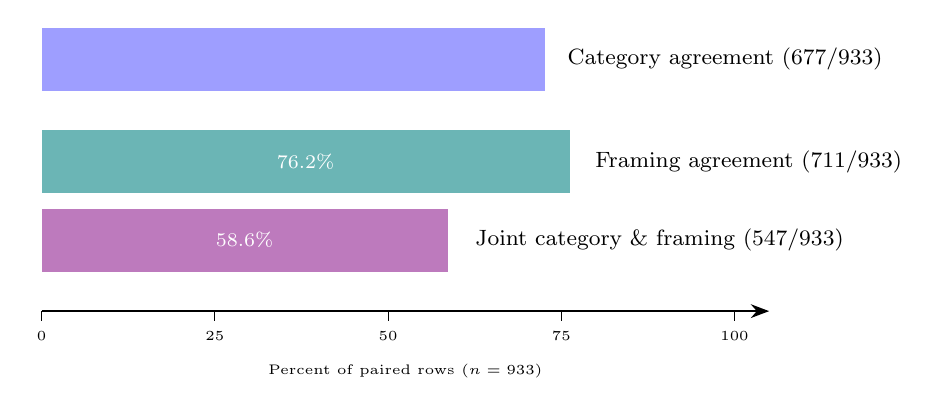
\begin{tikzpicture}[font=\footnotesize,x=0.088cm]
\draw[thick,-Stealth] (0,-0.45) -- (105,-0.45);
\foreach \x/\lab in {0/0,25/25,50/50,75/75,100/100}
  \draw (\x,-0.45) -- (\x,-0.58) node[below,font=\tiny]{\lab};
\node[below,font=\tiny,yshift=-12pt] at (52.5,-0.58) {Percent of paired rows ($n=933$)};
\fill[blue!38] (0,2.35) rectangle (72.6,3.15) node[midway,font=\scriptsize]{72.6\%};
\node[anchor=west,font=\footnotesize] at (74.5,2.75) {Category agreement ($677/933$)};
\fill[teal!58] (0,1.05) rectangle (76.2,1.85) node[midway,font=\scriptsize,text=white]{76.2\%};
\node[anchor=west,font=\footnotesize] at (78.5,1.45) {Framing agreement ($711/933$)};
\fill[violet!52] (0,0.05) rectangle (58.6,0.85) node[midway,font=\scriptsize,text=white]{58.6\%};
\node[anchor=west,font=\footnotesize] at (61.2,0.45) {Joint category \& framing ($547/933$)};
\end{tikzpicture}
\caption{Fixture-wide hit rates on paired rows after alignment: three marginal summaries that offset Figure~\ref{fig:mismatch_top}'s directional stress.}
\label{fig:fixture_agreement}
\end{figure}

\subsubsection{Segment length and disagreement}
Means conditioned on $\max(|\mathrm{entry\_eng}|,|\mathrm{entry\_rus}|)\ge 50$ stay matched across agreement flags (Step~D). Bucketed counts tell a finer story: short clauses dominate the memoranda, yet disagreement appears throughout the mass rather than clustering exclusively in the tail. The $100$--$199$ bucket remains thin ($20$ paired rows total here), so fluctuations there deserve cautious reading.

\begin{figure}[htbp]
\centering
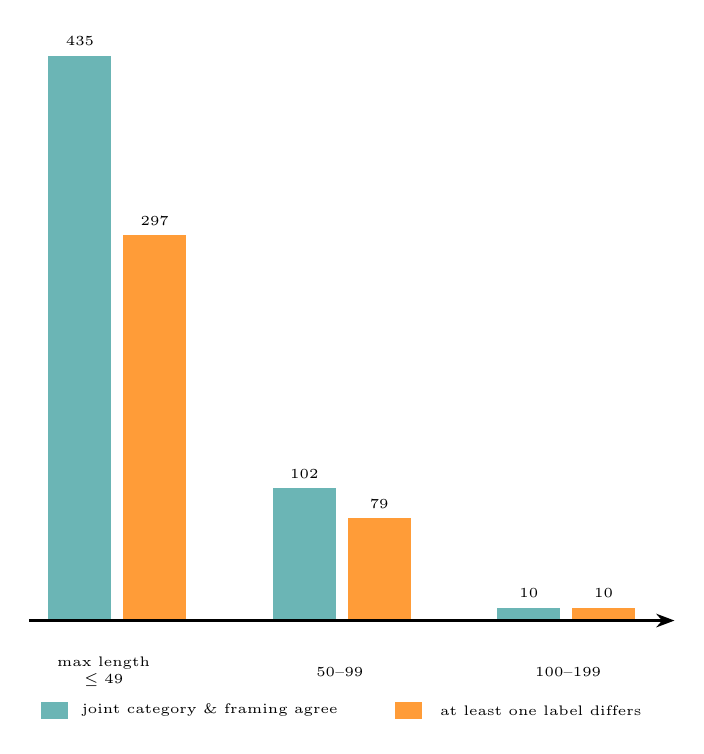
\begin{tikzpicture}[font=\footnotesize]
\begin{scope}[y={(0,0.0165)}]
  \fill[teal!58] (0.25,0) rectangle (1.05,435);
  \fill[orange!78] (1.2,0) rectangle (2.0,297);
  \node[font=\tiny,anchor=south] at (0.65,435) {$435$};
  \node[font=\tiny,anchor=south] at (1.6,297) {$297$};
  \fill[teal!58] (3.1,0) rectangle (3.9,102);
  \fill[orange!78] (4.05,0) rectangle (4.85,79);
  \node[font=\tiny,anchor=south] at (3.5,102) {$102$};
  \node[font=\tiny,anchor=south] at (4.45,79) {$79$};
  \fill[teal!58] (5.95,0) rectangle (6.75,10);
  \fill[orange!78] (6.9,0) rectangle (7.7,10);
  \node[font=\tiny,anchor=south] at (6.35,10) {$10$};
  \node[font=\tiny,anchor=south] at (7.3,10) {$10$};
\end{scope}
\draw[thick,-Stealth] (0,0) -- (8.2,0);
\node[font=\tiny,align=center] at (0.95,-0.65) {$\max$ length\\$\le 49$};
\node[font=\tiny,align=center] at (3.95,-0.65) {$50$--$99$};
\node[font=\tiny,align=center] at (6.85,-0.65) {$100$--$199$};
\begin{scope}[shift={(0.15,-1.25)}]
  \fill[teal!58] (0,0) rectangle (0.35,0.22);
  \node[anchor=west,font=\tiny] at (0.4,0.11) {joint category \& framing agree};
  \fill[orange!78] (4.5,0) rectangle (4.85,0.22);
  \node[anchor=west,font=\tiny] at (4.95,0.11) {at least one label differs};
\end{scope}
\end{tikzpicture}
\caption{Paired-row counts by coarse $\max(|\mathrm{entry\_eng}|,|\mathrm{entry\_rus}|)$ bucket: teal counts fully agreeing rows; orange counts rows with any category or framing mismatch (fixture totals match Step~D's long-clause means).}
\label{fig:length_mismatch_bins}
\end{figure}

\subsubsection{Lexical diversity as a separate axis}
Document-level English type-token ratios are orthogonal to the alignment ledger: they describe stylistic repetition across each memorandum's English surface, not paired-row accuracy. Figure~\ref{fig:ttr_axis} places that axis after structural diagnostics so ``easy-looking'' bulletins are not mistaken for semantically easy spans.

\begin{figure}[htbp]
\centering
\makebox[\linewidth][c]{%
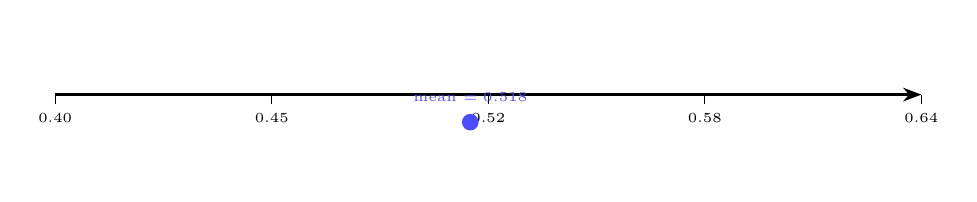
\begin{tikzpicture}[font=\footnotesize]
\pgfmathsetmacro{\ttrmn}{0.403}
\pgfmathsetmacro{\ttrmx}{0.643}
\pgfmathsetmacro{\ttrmean}{0.518}
\pgfmathsetmacro{\ttrspan}{\ttrmx-\ttrmn}
\path[use as bounding box] (-0.35,-1.0) rectangle (11.35,0.85);
\draw[thick,-Stealth] (0,0)--(11,0);
\foreach \x/\lbl in {0/0.40,2.75/0.45,5.5/0.52,8.25/0.58,11/0.64}
  \draw (\x,0)--(\x,-0.12) node[below,font=\tiny] {\lbl};
\pgfmathsetmacro{\dotx}{((\ttrmean-\ttrmn)/\ttrspan)*11}
\fill[blue!70] (\dotx,-0.35) circle (3pt) node[above=4pt,font=\tiny] {mean $=0.518$};
\end{tikzpicture}%
}
\caption{Lexical diversity landscape for the fixture (English surfaces): repetitive bulletins sit left, more heterogeneous memoranda sit right. Ratios use min token length $3$ with stopwords removed; document-level points span $0.403$--$0.643$.}
\label{fig:ttr_axis}
\end{figure}

\subsection{Interpretive role of the Research Lab charts}
Charts and tables both read the same comparison file produced after pairing: they show different slices of \emph{one} dataset, so a heatmap and a word cloud cannot contradict each other unless the export changed between builds. Chart.js draws the numeric panels; Voyant embeds show which phrases keep company across the whole corpus, outside our label menus \citep{sinclair2016voyant}. Treat Sections~\ref{sec:fixture_journey} and~\ref{sec:fixture_balance} as the rehearsal: once you know which cells dominate, which framing swaps concentrate, and where headline agreement still lands, each visualization answers a narrower follow-up question instead of introducing the corpus cold.

\subsubsection{Lexical and marginal distributions}
\textbf{Word clouds (English and Russian).} Tokens accumulate from segment surfaces after stopword removal with deterministic colouring so repeated renders stay comparable. \textit{Teaching move:} compare cloud asymmetry between languages on the same document id before blaming ``model confusion''; misaligned OCR spikes surface here first.

\textbf{Category $\times$ framing heatmap.} Cells count segments sharing both labels with intensity scaled to the modal cell. Cross-check Figure~\ref{fig:heatmap_topcells}: the ranked bars strip colour scaling away so you see literal counts behind the heatmap gradient.

\textbf{Per-document stacked bars and corpus pies.} Bars tally category or framing counts per memorandum; pies aggregate across loaded docs. Use bars to narrate single-file skew (one bulletin drenched in institutional framing), pies to calibrate rarity so Legal Framework slices are read with appropriate uncertainty.

\textbf{Terms-by-category and terms-by-framing horizontal bars.} Distinct bilingual surfaces count once even when boilerplate repeats. Use them to verify whether lemmas match expectations (legal stems under Legal Framework, evaluative adjectives under discrediting framings).

\textbf{Vocabulary diversity (type-token ratio).} Recall Figure~\ref{fig:ttr_axis}: $\mathrm{TTR}=\mathrm{types}/\mathrm{tokens}$ on English full-document text rescales to percentages in the UI. Low diversity means repetition, not necessarily low classification accuracy.

\textbf{Trends (line chart across documents).} Each polyline tracks category counts in catalogue order, not strict chronology; treat zig-zags as ingestion-order artefacts unless dates are merged manually.

\subsubsection{Agreement structure}
\textbf{Segment length versus matches.} Scatter coordinates use $\max(|\mathrm{entry\_eng}|,|\mathrm{entry\_rus}|)$ with jitter for matched versus mismatched paired rows; Section~\ref{sec:fixture_journey} already cited mean lengths near $73$ characters for long clauses, and Figure~\ref{fig:length_mismatch_bins} reports bucketed totals from the same fixture export; carry both when scanning plots.

\textbf{Mismatch flow matrix.} Rows fix model framing labels and columns fix expert framing labels for paired segments. Figure~\ref{fig:mismatch_top} isolates the three busiest arrows so you can read the full matrix without drowning in twenty-five cells.

\subsubsection{Geography and Voyant readers}
\textbf{Places map.} Leaflet markers scale with mention counts for Places-tagged segments; popups deep-link to segments when enrichment exists. Use maps when abstract place codes need geographic intuition.

\textbf{Voyant Cirrus, Links, Bubblelines, Constellations.} Hosted corpora reveal phrase attraction beyond taxonomy boundaries (committee titles, geographic compounds), serving as macro checks on heatmap concentration.

\subsubsection{Rhetorical similarity}
\textbf{Document fingerprints and cosine similarity.} Fingerprints chart framing mixtures; cosine compares normalized vectors so length-independent similarity peaks near one for rhetorical twins. The fixture peaks at $0.998$ between \texttt{1213.txt} and \texttt{1245.txt}, reinforcing that cosine proximity is not archival adjacency.

\textbf{Radar (category axes).} Compare documents radially when stacked bars feel too granular.

\textbf{Terms-by-framing lists and term$\times$framing heatmaps.} Dense intersections between evaluative lemmas and discrediting framings ground the linguistic theory behind framing codes.

\subsection{Reproducibility}
Section~\ref{sec:fixture_journey}'s integers were checked against the bundled sample shipped with the manuscript revision; Section~\ref{sec:fixture_balance}'s headline percentages and bucketed counts were recomputed from the same shipped JSON's \texttt{aligned\_rows}. If you regenerate the report from a new model run, treat those counts as illustrative until you reread the comparison tables they summarize.

% =============================================================================
\section{Outcomes and contribution}
\label{sec:outcomes}

The bundled fixture journey (Section~\ref{sec:fixture_journey}) makes one substantive empirical point easy to miss if readers jump straight to charts: most segments pair inventory-heavy categories with either ideological discrediting or institutional wrapping, so models face coupled tone-and-content recovery rather than neat factorization.

Dual coding therefore foregrounds asymmetric failures: cases where actors and dates look correct while ideological shading collapses into bureaucracy (Figure~\ref{fig:mismatch_top}), or where tone sounds plausible yet entities misattach. Evidence for those asymmetries always lives in paired comparison rows before it appears as shaded cells; Section~\ref{sec:fixture_balance} recalls headline agreement rates so those diagnostics stay tethered to how often marginal hits occur alongside swaps.

Practically, the repository contributes an evaluation harness for declassified memoranda with bilingual readers; an alignment layer whose greedy rules are spelled out in Section~\ref{sec:methods}; and an HTML report binding glossary definitions to highlighted passages so qualitative audit trails remain first-class.

Serving models locally via Ollama keeps payloads on-premises while exposing comparator code sufficient for replication. Natural extensions include richer automatic segmentation without expert spans, grammar-constrained JSON decoders, multi-way confusion summaries with chance correction \citep{cohen1960coefficient,carletta1996assessing}, and prompt comparisons screened with multiplicity-aware protocols \citep{benjamini1995controlling}.

% =============================================================================
\appendix

\section{Formal pipeline specification}
\label{app:formal}

Think of Appendix~\ref{app:formal}--\ref{app:compare} as the lookup sheet for symbols already introduced informally: each block states one claim about how records transform, gives the formal tuple or equation, then returns you to Section~\ref{sec:methods} for interpretation. Skip proofs on first reading unless you are reimplementing the comparator.

Throughout appendices $\Sig$ denotes finite strings of Unicode characters produced by transcripts or prompts (the Kleene closure of the alphabet $\Sigma$). Symbols $\mathcal{C}$ and $\mathcal{F}$ enumerate admissible content categories and framing strategies fixed by taxonomy $T$. Macros $\Pred$ and $\GT$ abbreviate prediction and expert-loading routines respectively.

\subsection{Ingest map}
Ingest expands catalogue indices into tuples carrying identifiers and text payloads. Formally $\mathrm{Ingest}(\mathcal{M}) = \{\phi(i): i\in\mathcal{M}\}$ with $\phi(i)=(\mathrm{id}_i,\mathrm{RUS}_i,\mathrm{ENG}_i,\ldots)$. Independent reimplementations should mirror $\phi$ so pairing keys stay aligned with shipped fixtures.

\subsection{Row space}
Each row bundles section metadata, bilingual spans, and labels drawn from finite taxonomy sets $\mathcal{C}$ (content) and $\mathcal{F}$ (framing):
$r\in\mathcal{S}=\mathrm{Section}\times\Sig\times\Sig\times\mathcal{C}\times\mathcal{F}\times\Sig.$
The trailing $\Sig$ slot holds auxiliary strings such as prose context surfaced in readers.

\subsection{Stub predictor}
Continuous-integration stubs fabricate ordering without semantic fidelity:
\[
\Pred_{\mathrm{stub}}(i)=\{(j,\varepsilon,p_j,c_{j\bmod m},f_{j\bmod n},p_j)\}_{j=1}^K,\quad m=|\mathcal{C}|,\ n=|\mathcal{F}|,\ K\le 25,\ |p_j|\ge 4.
\]
Indices $j$ impose fake positions while categories cycle modulo cardinalities purely for plumbing tests.

\subsection{Ollama predictor}
Neural extraction concatenates prompt templates with truncated Russian sources, then parses rows from returned text:
\[
\Pred_{\mathrm{LLM}}(i)=\mathrm{Parse}(\mathcal{A}_\theta(P_i)),\quad P_i=\mathrm{Prompt}(\pi_{8000}(\mathrm{RUS}_i),\mathcal{C},\mathcal{F}),
\]
with fallback to $\Pred_{\mathrm{stub}}$ when parsing fails. Here $\mathcal{A}_\theta$ denotes the served autoregressive model weights.

\subsection{Ground truth}
Experts may emit different counts per document: $\GT(i)=(g_1,\ldots,g_{n_i})\in\mathcal{S}^{n_i}$. Length $n_i$ need not equal machine row counts until alignment completes.

\subsection{Alignment}
Let $|G|=n_H$ and $|L|=n_L$. Define $\eta(s)=\mathrm{lower}(\mathrm{collapse}(\mathrm{strip}(s)))$ where $\mathrm{collapse}$ collapses internal whitespace runs (labels themselves compare under stripped equality without lowercasing). Greedy pairing yields $\mathcal{P}_i\subseteq\{1,\ldots,n_H\}\times\{1,\ldots,n_L\}$ with $|\mathcal{P}_i|\le\min(n_H,n_L)$, so unmatched rows contribute zero to agreement numerators.

\subsection{Accuracy}
Indicators $\mathrm{cat}(r)$ and $\mathrm{fram}(r)$ record stripped string equality between expert and predicted categories or framings (no case folding on labels). Section~\ref{sec:methods} averages those indicators over paired rows to match exported percentages bundled with HTML.

\section{LLM interface and neural decoding sketch}
\label{app:llm}

Readers tracing Figure~\ref{fig:l7a} alongside Section~\ref{sec:methods} need only two intuitions before the product formula: (i) logits rank vocabulary entries at each step; (ii) softmax turns logits into probabilities so sampling can draw the next token. Everything else is mechanical detail for implementers.

Let tokens be integers drawn from a finite vocabulary; a prefix $z_{1:L}$ seeds generation. Autoregressive models factorize the conditional probability of completing the suffix $z_{L+1:T}$ as a product of next-token probabilities \citep{vaswani2017attention}:
\[
p_\theta(z_{L+1:T}\mid z_{1:L})=\prod_{t=L}^{T-1}p_\theta(z_{t+1}\mid z_{1:t}).
\]
Each factor asks ``given everything generated so far, how likely is each vocabulary entry as the very next token?'' Multiplying factors yields the joint probability of an entire completion because earlier choices influence later logits through hidden states.

Transport failures map to a sentinel $\bot$ via $\mathrm{HTTP}_\theta:\Sig\to\Sig\cup\{\bot\}$ so parsers distinguish empty models from network errors. At decode step $t$, logits $u_t$ become a probability vector via $\mathrm{softmax}(u_t/\tau)$: exponentiating entries, dividing by temperature $\tau$ (larger $\tau$ flattens peaks), and normalizing so every probability is nonnegative and sums to one. Sampling or argmax-selecting from that vector chooses $z_{t+1}$; Figures~\ref{fig:l7a}--\ref{fig:l7c} depict client routing and the loop with optional caps $M$.

\begin{figure}[htbp]
\centering
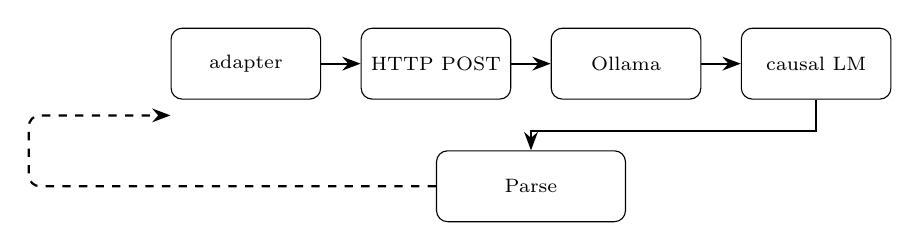
\begin{tikzpicture}[font=\scriptsize,
  box/.style={draw,rounded corners,minimum height=9mm,minimum width=19mm,align=center},
  arr/.style={-{Stealth},thick},
  rarr/.style={-{Stealth},thick,dashed}]
\node[box] (bxAda) {adapter};
\node[box,right=5mm of bxAda] (bxHttp) {HTTP POST};
\node[box,right=5mm of bxHttp] (bxOll) {Ollama};
\node[box,right=5mm of bxOll] (bxLm) {causal LM};
\coordinate (belowlm) at ($(bxHttp.south)!0.5!(bxOll.south)+(0,-11mm)$);
\node[box,minimum width=24mm] (bxParse) at (belowlm) {Parse};
\draw[arr] (bxAda.east)--(bxHttp.west);
\draw[arr] (bxHttp.east)--(bxOll.west);
\draw[arr] (bxOll.east)--(bxLm.west);
\draw[arr] (bxLm.south) -- ++(0,-4mm) -| (bxParse.north);
\coordinate (leftlane) at ($(bxAda.west)+(-18mm,0)$);
\draw[rarr,rounded corners]
  (bxParse.west) -- (leftlane |- bxParse.west)
  |- ([yshift=-2mm]bxAda.south west);
\end{tikzpicture}
\caption{Client--server boundary; dashed path returns parsed rows.}
\label{fig:l7a}
\end{figure}

\begin{figure}[htbp]
\centering
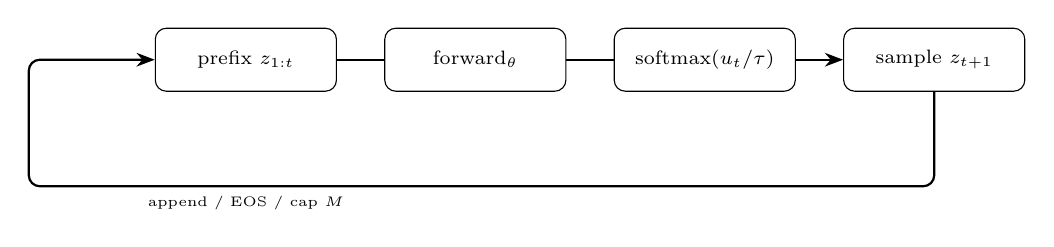
\begin{tikzpicture}[font=\scriptsize,
  box/.style={draw,rounded corners,inner sep=3pt,minimum height=8mm,minimum width=23mm,align=center},
  arr/.style={-{Stealth},thick},
  >=Stealth]
\node[box] (bxZ) {prefix $z_{1:t}$};
\node[box,right=6mm of bxZ] (bxF) {forward$_\theta$};
\node[box,right=6mm of bxF] (bxS) {$\mathrm{softmax}(u_t/\tau)$};
\node[box,right=6mm of bxS] (bxSm) {sample $z_{t+1}$};
\draw[arr] (bxZ)--(bxF)--(bxS)--(bxSm);
\draw[arr,rounded corners]
  (bxSm.south) -- ++(0,-12mm)
  -| ($(bxZ.south west)+(-16mm,0)$)
  |- (bxZ.west);
\node[font=\tiny,align=center,below=2mm of bxZ,yshift=-10mm] {append / EOS / cap $M$};
\end{tikzpicture}
\caption{Autoregressive decode loop with temperature $\tau$ and token cap.}
\label{fig:l7c}
\end{figure}

\section{Compare module proofs}
\label{app:compare}

Lemma~\ref{lem:eta} reassures you that repeating normalization does not oscillate strings, which matters because pairing caches rely on stable keys. Theorems~\ref{thm:partial}--\ref{thm:acc} are bookkeeping: they guarantee exported denominators cannot invent extra partners and that ``both correct'' cannot exceed either marginal accuracy.

\begin{lemma}[Idempotence]
\label{lem:eta}
For all $s\in\Sig$, $\eta(\eta(s))=\eta(s)$.
\end{lemma}

\paragraph{Algorithm $\mathcal{A}$.}
Phase~A pairs rows whose $\eta$-images match exactly; Phase~B pairs strict containment cases where the shorter normalized span has length at least four characters.

\begin{theorem}[Partial matching]
\label{thm:partial}
Each GT index and LLM index receives at most one partner; $|P|\le\min(n_H,n_L)$.
\end{theorem}
\begin{proof}
Pairs consume endpoints; reuse forbidden.
\end{proof}

\begin{theorem}
\label{thm:acc}
For $m>0$ paired rows, reported accuracies lie in $[0,100]$; $\mathrm{Acc}^{\mathrm{both}}\le \min(\mathrm{Acc}^{\mathrm{cat}},\mathrm{Acc}^{\mathrm{fram}})$.
\end{theorem}
\begin{proof}
For each paired row $j$, let $C_j,F_j,B_j\in\{0,1\}$ be category match, framing match, and both-match indicators. By definition $B_j=C_j F_j\le C_j$ and $B_j\le F_j$. Summing over $m$ pairs and dividing by $m$ yields $\overline{B}\le \min(\overline{C},\overline{F})$; reported percentages scale by $100$.
\end{proof}

\section{Experiment-methods primer}
\label{app:primer}

\textbf{How to use this primer.} Return here after walking Figures~\ref{fig:error_sources} and~\ref{fig:reading_loop}: each bullet translates a visualization temptation into a statistical caveat referenced elsewhere in the paper.

\textbf{Units.} Segments nest inside documents; treating each segment as independent ignores shared authorship and duplicated boilerplate, so confidence intervals computed under i.i.d.\ assumptions misstate uncertainty.

\textbf{Multiplicity.} Interactive dashboards tempt analysts to mine whichever chart looks significant; Benjamini--Hochberg adjustments or pre-registered hypotheses supply disciplined alternatives \citep{benjamini1995controlling}.

\textbf{$\kappa$ versus accuracy.} When labels are skewed (many neutral framings, few ideological tags), percent accuracy can exceed chance dramatically even when raters disagree rarely but systematically on minority codes; Cohen's $\kappa$ subtracts expected agreement under marginal frequencies \citep{cohen1960coefficient,carletta1996assessing}.

\textbf{Lineage.} Neural decoding injects randomness whenever sampling non-argmax tokens, yet comparison and reporting remain deterministic functions of decoded strings plus expert rows \citep{norton2026ocrprovenance}. Tracking ``who introduced variability'' clarifies whether discrepancies warrant reruns versus comparator edits.

\begin{figure}[htbp]
\centering
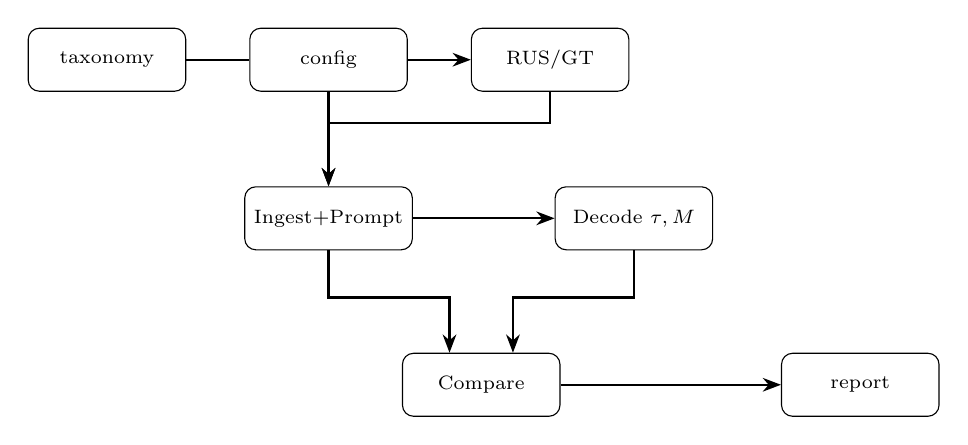
\begin{tikzpicture}[font=\scriptsize,
  box/.style={draw,rounded corners,minimum width=20mm,minimum height=8mm,align=center},
  arr/.style={-{Stealth},thick}]
\node[box] (tx) {taxonomy};
\node[box,right=8mm of tx] (cf) {config};
\node[box,right=8mm of cf] (ru) {RUS/GT};
\node[box,below=12mm of cf] (ip) {Ingest+Prompt};
\node[box,right=18mm of ip] (dc) {Decode $\tau,M$};
\coordinate (midrow) at ($(ip.south)!0.5!(dc.south)$);
\node[box,below=13mm of midrow] (cm) {Compare};
\node[box,right=28mm of cm] (rp) {report};
\draw[arr] (tx)--(cf)--(ru);
\draw[arr] (cf)--(ip);
\draw[arr] (ru.south) -- ++(0,-4mm) -| (ip.north);
\draw[arr] (ip)--(dc);
\draw[arr] (ip.south) -- ++(0,-6mm) -| ($(cm.north west)!0.3!(cm.north east)$);
\draw[arr] (dc.south) -- ++(0,-6mm) -| ($(cm.north west)!0.7!(cm.north east)$);
\draw[arr] (cm)--(rp);
\end{tikzpicture}
\caption{Lineage: stochastic decode vs deterministic comparison/reporting.}
\label{fig:lineage}
\end{figure}

\section{Plain-language companion}
\label{app:plain}

This appendix restates project ideas without statistical jargon. Read it alongside Section~\ref{sec:task} and the HTML report itself.

\subsection{What the software is for}
Historians label short quotations from memoranda with two kinds of tags. The goal here is to check whether an automated assistant can propose the same tags as the experts \emph{and} to publish tables and charts so any reader can see mismatched quotations alongside definitions. The grand payoff is transparency on sensitive archives: headline percentages never substitute for reading the clause.

\subsection{What a segment row is}
Think of a spreadsheet row: one quotation from Russian text (sometimes paired with English), plus two dropdown answers chosen from fixed menus (what topic bucket it belongs to: Actors, Places, etc.; and how it sounds politically or stylistically: neutral, bureaucratic, ideological,\ldots). Every downstream chart ultimately counts or compares those rows.

\subsection{Why there are two labels}
Police memoranda often list facts while implying suspicion or loyalty through wording alone. Separating ``what is mentioned'' from ``how it is said'' keeps analyses faithful to how archivists read sources rather than forcing everything into one noisy category.

\subsection{What ingest means here}
In plain terms: the program finds the right manuscript files listed in the project catalogue and bundles identifiers plus Russian (and optional English) text so later stages never chase stray filenames manually.

\subsection{What prediction means here}
Prediction is any pathway that fills machine-side spreadsheet rows: either an LLM (often via Ollama locally), a throwaway splitter used only for plumbing tests, or merged assessments exported after blind reviews.

\subsection{What comparison really checks}
Comparison asks ``did we attach model guesses to the \emph{same} Russian quotation as the expert row \emph{and} did both dropdown answers match character-for-character after trimming spaces?'' If the quotations differ because of paraphrase or split boundaries, pairing fails even when a human would agree with the model's intent.

\subsection{What the JSON export is}
It is the frozen snapshot of paired rows and match flags that both the HTML tables and Research Lab charts consume. If two visuals disagree, they should still trace back to the same JSON row ids; otherwise something is misconfigured.

\subsection{What charts help with (and what they cannot do)}
Charts summarize frequency patterns (which topics dominate, which framing swaps recur, how diverse English prose is). They cannot prove archival facts by themselves; they point your eye toward quotations worth reopening in Voyant or bilingual panels.

\subsection{Fixture numbers in one breath}
The bundled sample dataset mentioned throughout Section~\ref{sec:fixture_journey} contains sixteen documents and 933 counted segments; its hottest joint labels involve actors paired with ideological or bureaucratic framing; the biggest framing disagreements pit bureaucratic model tags against action-focused expert tags. Those specifics exist so prose stays tethered to reproducible counts rather than intuition alone.

\section{Passages reviewers flagged as jargon-prone}
\label{app:jargon_list}

The following locations still lean on specialist shorthand and deserve another plain-language pass tied to Appendix~\ref{app:plain}:
\begin{enumerate}[leftmargin=*]
  \item \textbf{Related work (both paragraphs):} Cohen $\kappa$, multiplicity control, and transformer decoding references assume readers know why those citations appear beside archival tooling.
  \item \textbf{Abbreviations table (symbols block):} Greek symbols and composition notation remain opaque without rereading Section~\ref{sec:methods}.
  \item \textbf{Ingestion subsection:} phrases such as ``anchor token surfaces'' hide the simple claim ``Russian files drive matching keys.''
  \item \textbf{Prediction bullets (Ollama path):} ``model logits,'' ``parse time,'' and $\pi_{8000}$ need either intuition boxes or pointers to Appendix~\ref{app:plain}.
  \item \textbf{Ground-truth alignment paragraph:} greedy matching versus Hungarian assignment trades transparency for optimality; readers may miss why we accept suboptimal pairing.
  \item \textbf{Metrics subsection opening:} ``conjunction (both match)'' compresses how exported percentages are averaged.
  \item \textbf{Fixture journey Step B--F:} rhetoric such as ``coupled tone-and-content recovery'' should echo simpler wording about simultaneous labeling tasks.
  \item \textbf{Interpretive role subsection headers:} ``orthogonal to taxonomy slices'' should name Voyant's concrete affordance (phrase collocations outside label menus).
  \item \textbf{Outcomes section middle paragraph:} ``asymmetric failures'' benefits from an everyday example already shown in Figure~\ref{fig:mismatch_top}.
  \item \textbf{Formal appendix blocks:} tuples $\mathcal{S}$, modulo arithmetic in stub equations, and HTTP$_\theta$ maps remain implementer-facing unless paired with Appendix~\ref{app:plain}.
  \item \textbf{LLM appendix product formula:} probability products intimidate non-ML readers despite the preceding intuition paragraph.
  \item \textbf{Compare proofs:} lemmas and inequalities reassure engineers more than historians; cross-link to the ladder figure when revising.
\end{enumerate}

\bibliographystyle{plainnat}
\bibliography{references}

\end{document}
